\chapter{Fields}
[TODO: revisit title so it's clear what's in Ch. 3 vs. 4 vs. 5]

In many applications, the heap is filled mostly with instances of just a
few important classes.  You can increase scalability significantly by making these
objects as compact as possible. This chapter describes field usage
patterns that can be easily optimized for space, for example, fields that are
rarely needed, constant fields, and dependent fields. Simple refactoring of
these kinds of fields can sometimes result in big wins.
 

\section{Rarely Used Fields: Using Side Objects}
\label{sec:rarely-used}

Chapter~\ref{chapter:delegation} presents examples where delegating fields
to another class increases memory cost. However, sometimes delegation can
actually save memory, if you don't have to allocate the delegated object all the
time.

As an example, consider an on-line store with millions of products. 
Most of the products are supplied by the parent company, but
sometimes the store sells products from another company:
\begin{shortlisting} 
class Product {
	String sku;
	String name;
	..
	String alternateSupplierName;
	String alternateSupplierAddress;
	String alternateSupplierSku;
}
\end{shortlisting}
When there is no alternate supplier, the last three fields
are never used. By moving these fields to a separate side class, you can
 save memory, provided the side object is allocated only when
it is actually needed. This is called \emph{lazy allocation}. Here are the 
refactored classes:

\begin{shortlisting} 
class Product {
	String sku;
	String name;
	.. 
	Supplier alternateSupplier;
}

class Supplier {
	String supplierName;
	String supplierAddress;
	String sku;
}
\end{shortlisting}
For products with no alternate supplier, eight bytes are saved per product,
since three fields are replaced by one. Of course, products with an alternate
supplier pay a delegation cost, including an extra pointer and object header.
An interesting question is how much total memory is actually saved? The
answer depends on the percentage of products that have an alternate supplier and
need
a side object, which we'll call the \emph{fill rate}. The higher the fill rate, the less memory is 
saved. In fact, if the fill rate is too high, memory is wasted.

Figure~\ref{fig:fill-rate} shows the average memory saved for different
fill rates, assuming three fields (12 bytes) are delegated. The most memory that can be
saved is 8 bytes, or 67\% of the bytes moved to the side object, when the fill
rate is 0\%.
When the fill rate is 10\%, 50\% of memory is saved.
When the fill rate is over 40\%, the memory saved is
negative, that is, memory is wasted. The lesson here is that if you aren't sure
what the fill rate is, then using delegation to save memory may end up
backfiring.
\begin{figure}
  \centering
 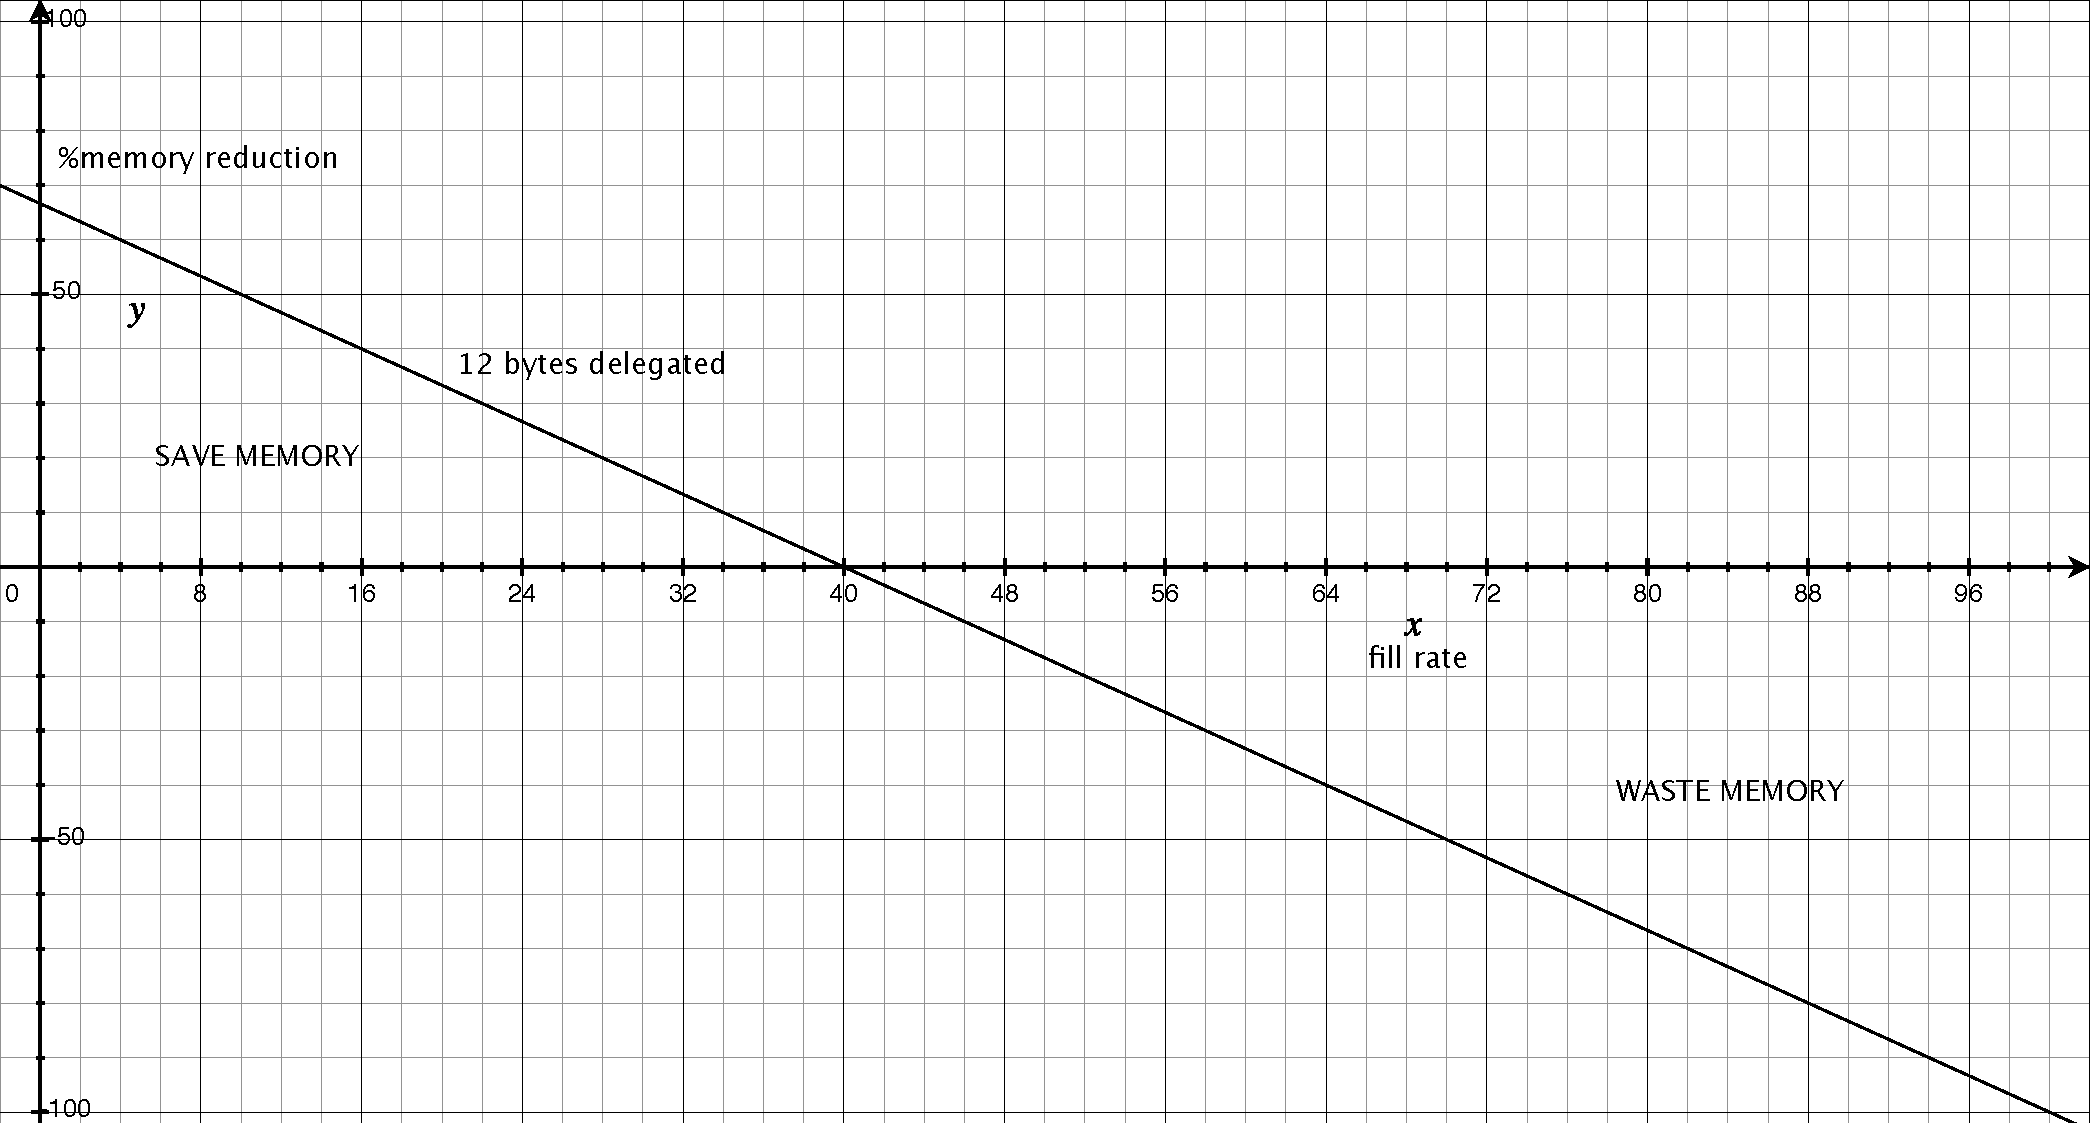
\includegraphics[width=.90\textwidth]{part1/Figures/modelingdatatypes/12-byte-graph.pdf}
 % 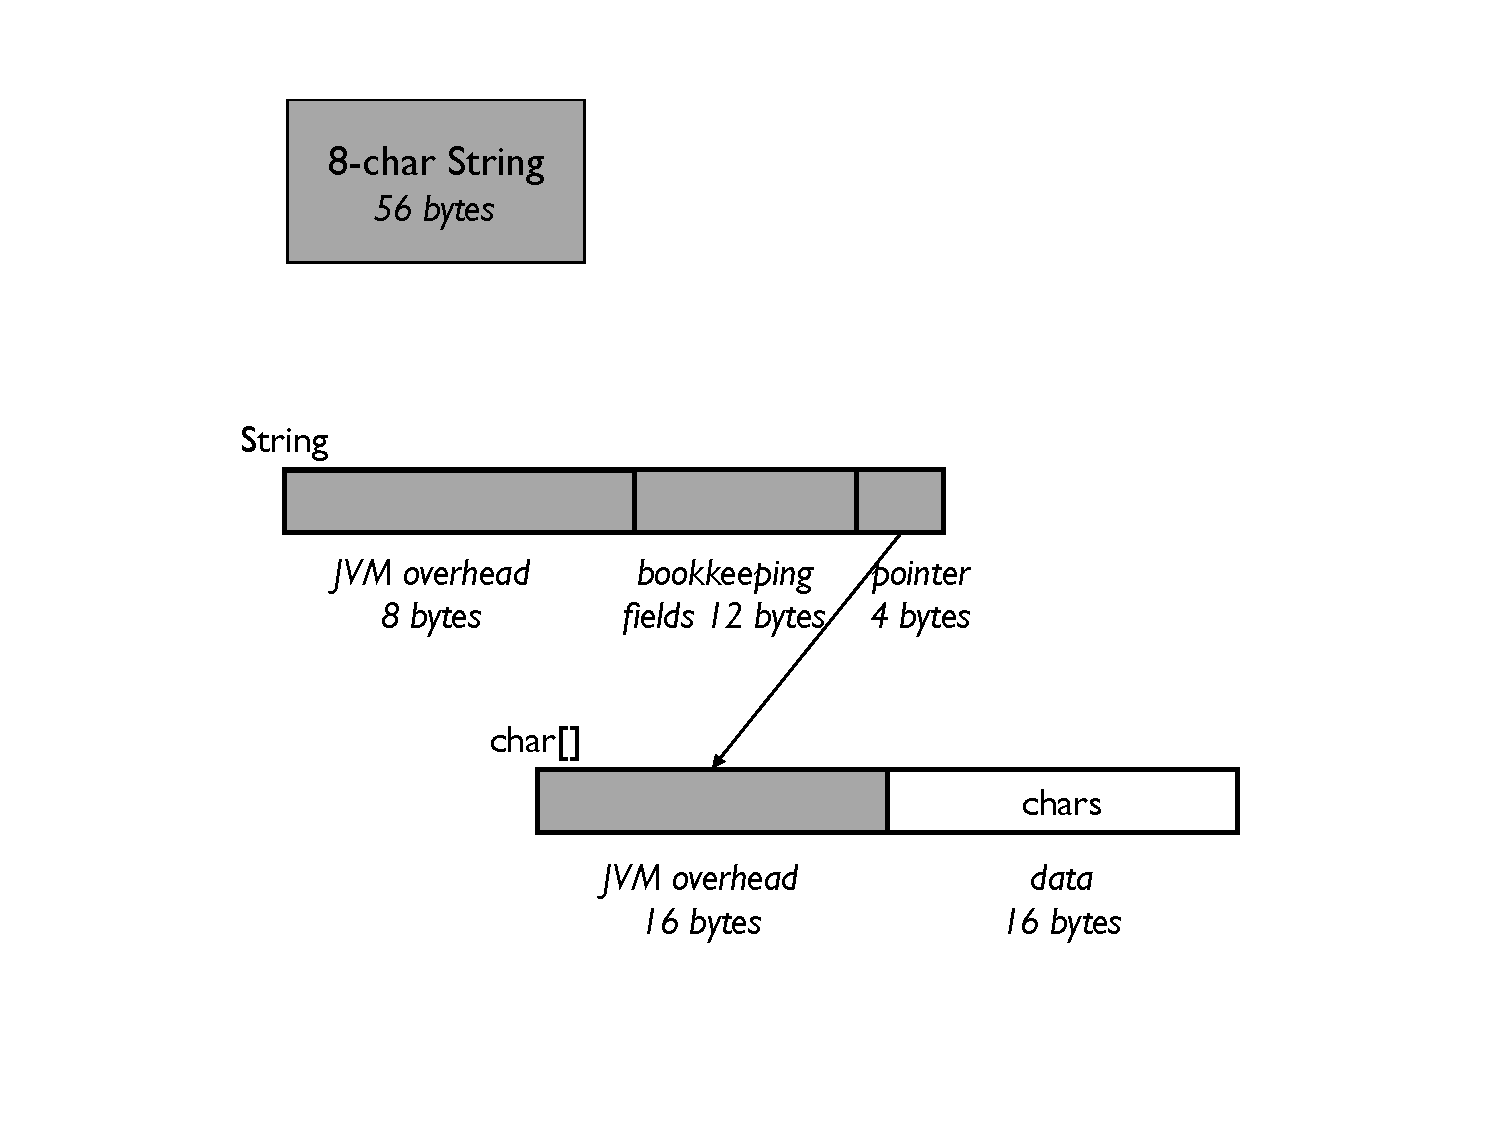
\includegraphics{eight-char-string}
  \caption{This plot shows how much memory is saved or wasted by delegating 12
  bytes of memory to a side object. The x-axis is the fill rate, and the
  y-axis is the percent of memory saved.}
  \label{fig:fill-rate}
\end{figure}

In addition to the fill rate, the memory savings also depends on the
number of fields delegated and their sizes. The more bytes delegated,
the larger the memory savings, assuming the same fill rate. Figure~\ref{fig:rarely-used} shows the memory
saved for different fill rates and sizes of delegated fields. Each
line represents a different delegated-field size. The bottom-most line
represents a delegated field size of 16 bytes, the next line represents 32 bytes, the next
represents 48 bytes, and so on, up to 144 bytes. As the delegated object size
increases, you can worry less about the fill rate. For example, if 32 bytes
are delegated, there is almost 90\% savings with a low fill rate, and some
memory savings with a fill rate up to 70\%. As the delegation size increases, 
the lines start to converge, since the delegation cost becomes relatively
less important.
\begin{figure}
  \centering
 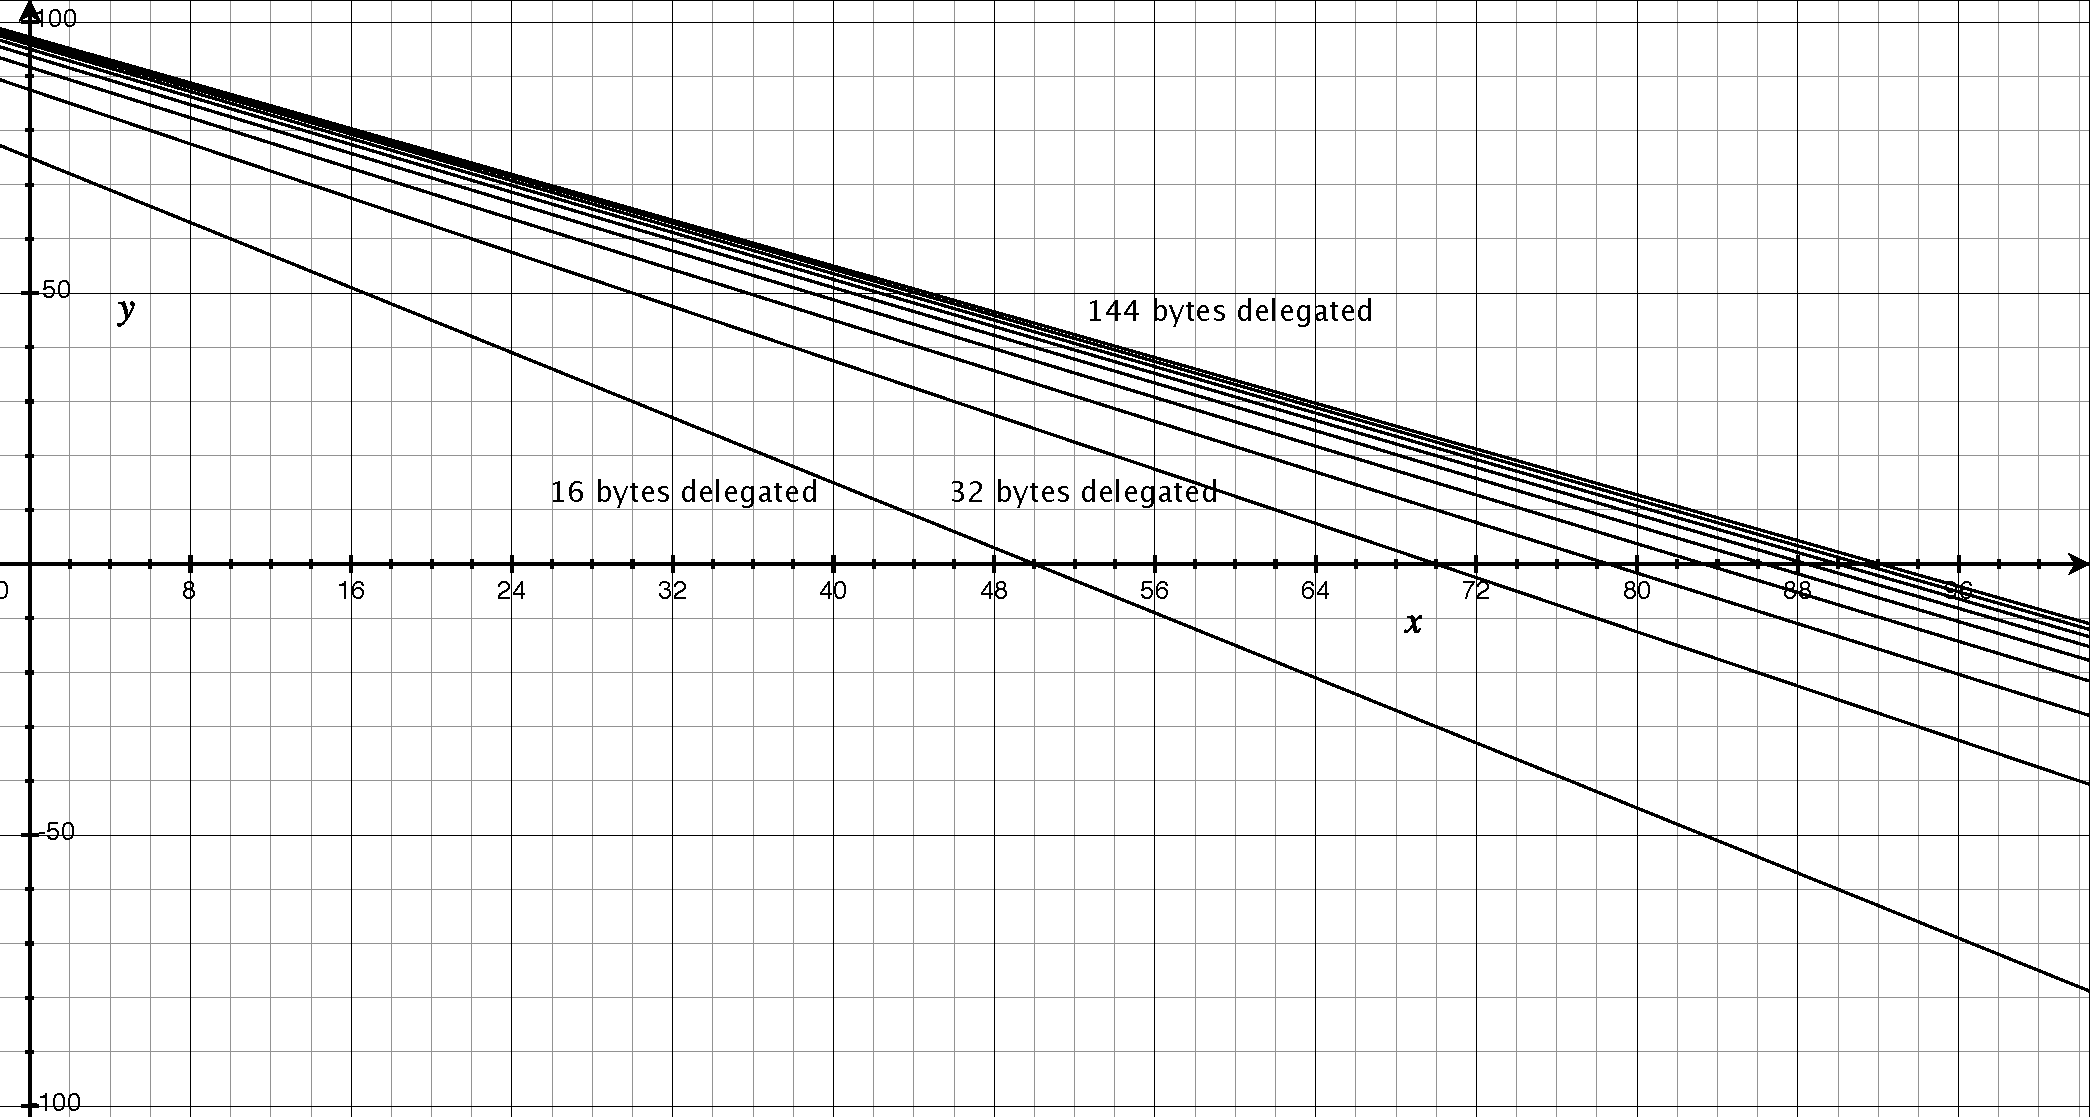
\includegraphics[width=.90\textwidth]{part1/Figures/modelingdatatypes/rarely-used.pdf}
 % 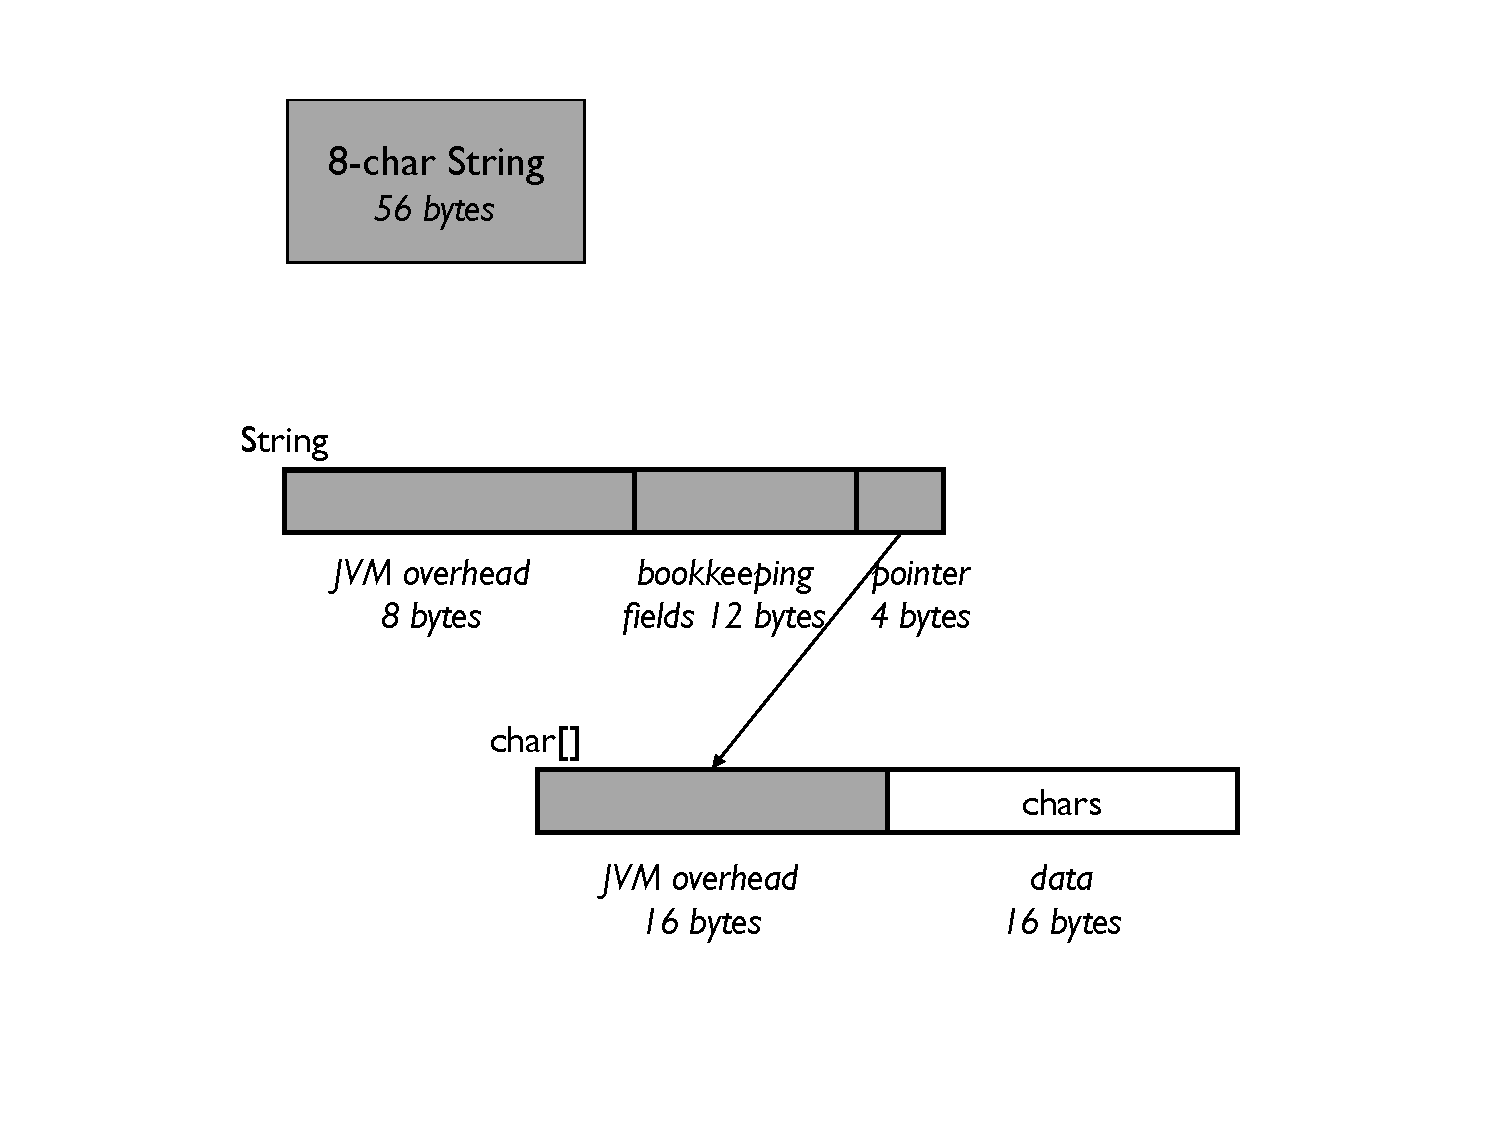
\includegraphics{eight-char-string}
  \caption{The amount memory saved or wasted is dependent on the
  size of the delegated fields and on the fill rate.
  The x-axis is the fill rate as a percent; the y-axis is the percent of
  memory saved on average, relative to the bytes delegated. Each line shows
  a different delegated size, from 16 bytes to 144
  bytes in increments of 16 bytes.}
  \label{fig:rarely-used}
\end{figure}

\callout{callout:rarely-used}{Delegation Savings Calculation}{
\index{Delegation Cost Calculation}
Assume the cost of a pointer is 4 bytes, and the cost of an object header is 8
bytes, and
\begin{eqnarray} 
B &=& the\ size\ in\ bytes\ of\ the\ delegated\ fields \nonumber \\
F &=& the\ fill\ rate,\ between\ 0\ and\ 1 \nonumber
\end{eqnarray}
Every main object pays for an extra pointer in this design, and F
of them require a side object. The average savings across all of
the objects is the savings in the main objects minus the cost of the side
objects\footnote{This calculation does not take alignment costs into
account. Depending upon the other fields in your object, this can
increase the cost of delegating some fields to a side object.
On a JRE where the header size is not a multiple of the object alignment
(e.g.the IBM 32-bit JRE), the delegated design can also result in a smaller 
expenditure on alignment costs in some cases.}:
\begin{eqnarray}
Average\ savings\ &=& B-4\ \ -\ \ F(B+8) \nonumber
\end{eqnarray}
It is worth moving the fields to a side object when you have
confidence that the savings will be positive, when:
\begin{eqnarray}
F &<& \frac{B-4}{B+8} \nonumber
\end{eqnarray}
} 
A common error is to put rarely-used fields in a side
class with lazy allocation, and have some code paths that
cause the side object to be allocated all the time.
In this case, instead of saving memory, you pay the full cost of delegation as well as 
the cost of unused fields. 
Lazy allocation
can be error-prone, since it may require testing whether the object
exists at every use. In applications with concurrent access to the data, extra care is
required. This complexity has to be weighed against potential memory savings.

\section{Rarely-Used Fields: Using Attribute Tables}

If a field is very rarely used, then it might make sense to delete it from
its class altogether, and store it in a separate attribute table that maps objects to the attribute
values. For example, suppose that a few of the products have won major awards,
and you want to record this information. Rather than maintaining a field
\code{majorAward} in every product, you can define a table:

\begin{shortlisting}
class Product {
    static HashMap<String, String> majorAward = new HashMap();
    ..
}
\end{shortlisting}

Even though a \class{HashMap} has it's own high overhead, this design will come
out ahead if there are a small number of major awards. 
Whenever you add any kind of new table like this, however, you have to be
careful you do not introduce a memory leak. If products are garbage collected, 
the corresponding entries in the attribute table should be cleaned up. This
topic is discussed at length in ???.

\section{Constant Fields}
\label{sec:constant}

Declaring a constant field \code{static} is a simple way to
save memory. Programmers usually remember to make constants like \emph{pi} 
static. There are other situations that are a bit more subtle, for example,
when a field is constant because of how it is used in the context of an
application.

Returning to the product example, suppose that each product has a field
\code{catalog} that points to a store catalog.
If you know that there is always just one store catalog, then the field
\code{catalog} can be turned into a static, saving 4 bytes per product.

As a more elaborate example, suppose that a \class{Product} has a field
referencing a \class{Category} object, where a category may be
books, music, clothes, toys, etc.
Clearly, different products belong to different categories.
However, suppose we define
subclasses \class{Book}, \class{Music}, and \class{Clothing} of \class{Product}, 
and all instances of a subclass belong to the same category.  
Now the \code{category} field has the same value for products in each subclass,
so it can be declared static:

\begin{shortlisting} 
class Book extends Product {
	static Category bookCategory; 	// points to the book category object  
	..
}

class Music extends Product {
	static Category musicCategory;  // points to the music category object
	..
}

class Clothing extends Product {
	static Category clothingCategory;  // points to the clothing category object
	.. 
}
\end{shortlisting}

Knowing the context of how objects are created and used, and how they relate to
other objects, is helpful in making these kinds of memory optimizations.


\section{Mutually Exclusive Fields}
\label{sec:mutually-exclusive}

Sometimes a class has fields that are never used at the same time, and therefore
they can share the same space. Two mutually exclusive fields can be conflated
into one field if they have the same type. 
Unfortunately, Java does not have anything like
a union type to combine fields of different types. However, if it makes sense,
mutually exclusive field types can be broadened to a common base type to
allow this optimization. 

For example, suppose that each women's clothing product has a size, and there
are different kinds of sizes: xsmall-small-medium-large-xlarge,
numeric sizes, petite sizes, and large women's sizes. One way
to implement this is to introduce a field for each kind of size:
\begin{shortlisting}
class WomensClothing extends Product {
	static Category clothingCategory;  // points to the clothing category object
	..
	SMLSize     smlSize;
	NumericSize  numSize;
	PetiteSize   petiteSize;
	WomensSize   womensSize; 
}
\end{shortlisting}
Each type is an enum class, such as:
\begin{shortlisting}
enum SMLSize {
	XSMALL, SMALL, MEDIUM, LARGE, XLARGE;
}

enum NumericSize {
	ZERO, TWO, FOUR, SIX, EIGHT, TEN, TWELVE, FOURTEEN, SIXTEEN;
}

enum PetiteSize {
    ZERO, TWO, FOUR, SIX, EIGHT, TEN, TWELVE, FOURTEEN, SIXTEEN;
}

enum WomensSize {
	ONEX, TWOX, THREEX, FOURX;
}
\end{shortlisting}
These four size fields are mutually exclusive --- a clothing item cannot
have both a petite size and a women's size, for example. Therefore, you can
replace these fields by one field, provided that the four enum types are
combined into one enum type:
\begin{shortlisting}
class Clothing extends Product {
	static Category clothingCategory;  // points to the clothing category object
	..
	ClothingSize     size; 
}

enum ClothingSize {
	XSMALL, SMALL, MEDIUM, LARGE, XLARGE, 
	ZERO, TWO, FOUR, SIX, EIGHT, TEN, TWELVE, FOURTEEN, SIXTEEN,
    PETITE_ZERO, PETITE_TWO, PETITE_FOUR, PETITE_SIX, PETITE_EIGHT, PETITE_TEN,
    PETITE_TWELVE, PETITE_FOURTEEN, PETITE_SIXTEEN,
	ONEX, TWOX, THREEX, FOURX;
}

\end{shortlisting}

If the types of two mutually exclusive fields are different classes, then you
generalize these types by defining a common superclass, if possible. As a last
resort, you can always combine these fields into a single field of type
\class{Object}. Finally, if there are sets of fields that are mutually exclusive, then you can
define a side class for each set of fields, where all side classes have
a common superclass. In this case, you need to do the math to make sure that you
actually save memory, given the extra cost of delegation.

\section{Redundant Fields}

A field is redundant if it can be computed on the fly from other fields, and, in
principle, can be eliminated. In the simplest case, two fields store the same
information but in different forms, since the two fields are used for
different purposes. For example, product IDs are
more efficiently compared as \code{ints}, but more easily printed as
\code{Strings}. Since it is possible to convert one representation into the
other, storing both representations is not necessary, and only makes sense if
there is a real cost penalty from performing the data conversion.
In the more general case, a field may depend on many other values. For example,
you could allocate a field to store the number of items in a shopping cart,
 or simply compute it by adding up all of the shopping cart items. 

There is a trade-off between the performance cost of a conversion or computation
and the memory cost of an extra field, which has to be weighed in context. 
How often is the information needed and how expensive is it to compute? What's
the total memory cost? Comparing performance cost to memory cost is a bit like apples and oranges, 
but often it is clear which resource is most constrained. Here are several
considerations to keep in mind:
\begin{itemize}
  \item Redundant \class{String} fields should be avoided, since
strings have a very high overhead in Java, 
as we have seen.  
\item Computed fields are very useful when storing partial values avoids 
expensive quadratic computation. For example, if you need to support finding the
number of children of nodes in a graph, then caching
this value for each node is a good idea. 
\end{itemize}

\section{Large Base Classes and Fine-grained Designs}
\index{Base Class Baggage}

As discussed in the previous chapter, highly-delegated data models can result in
too many small objects. Occasionally, you run across a highly-delegated data model where the delegated objects
are large. This can happen when delegated classes inherit from a large base class. When fine grained data modeling
is combined with inheriting from large base classes, memory costs multiply and can become prohibitive.

%\begin{example}{Keeping track of updates} 
A frequent data management requirement is to track creation and update information, that is, when data is created or updated and by whom.  Here is a base class, taken from a real application, that stores create and update information.  
\begin{shortlisting}
class UpdateInfo {
     Date creationDate;
     Party enteredBy;
     Date updateDate;
     Party updatedBy;
}
\end{shortlisting}
You can track changes by subclassing from \class{UpdateInfo}. Update tracking is
a \textit{cross-cutting feature}, since it can apply to any class in a data model.
%\end{example}

Returning to the original, unoptimized
version of \class{EmployeeWithEmergencyContact} in
Section~\ref{fine-grained-data-models}, suppose that updates to employee emergency contacts need to be tracked. 
You need to decide how fine the tracking should be. Should every update to every
phone number and email address be tracked, or is it sufficient to track the fact that some
contact information was changed for an emergency contact? If you decide to
track changes to every contact phone number or email address, you can easily achieve this by
extending the \class{ContactMethod} class defined in the fine-grained data model from Section~\ref{fine-grained-data-models}:
\begin{shortlisting}
class ContactMethod extends UpdateInfo {
     ContactPerson owner;
}
\end{shortlisting}
Figure~\ref{fig:big-base-class} shows an instance of a contact person with
update information associated with every \class{ContactMethod}. Not only is this
a highly delegated structure with multiple \class{ContactMethod} objects, but
each one has an additional 16 bytes. Furthermore, there are potentially four
more objects of type \class{Date} and \class{Party} for each of the four
\class{ContactMethod} objects. A far more scalable solution is to move up a
level, and track changes to each \class{ContactPerson}. With this solution, you
do not need such a fine-grained data model, and the update tracking functionality is 1/4 the cost.
\begin{figure}
  \centering
 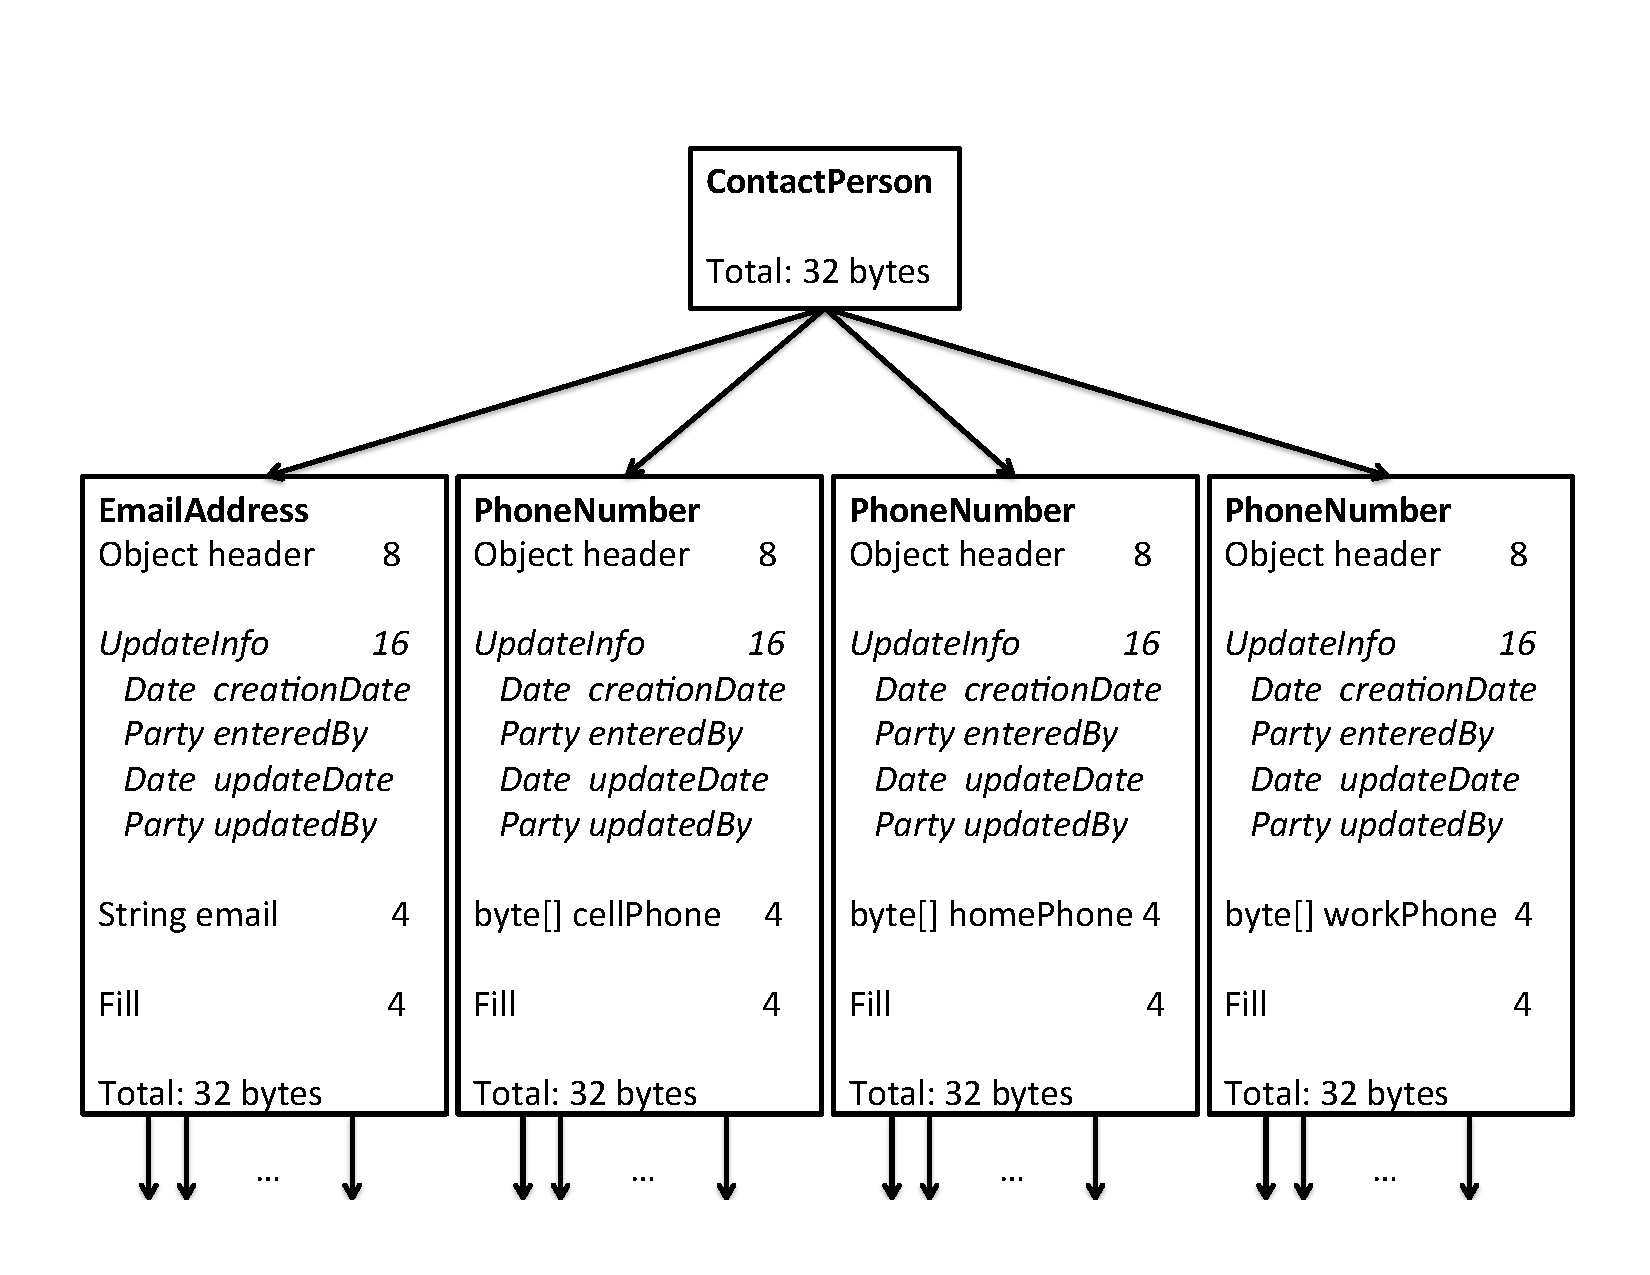
\includegraphics[width=.70\textwidth]{part1/Figures/modelingdatatypes/big-base-class.pdf}
 % 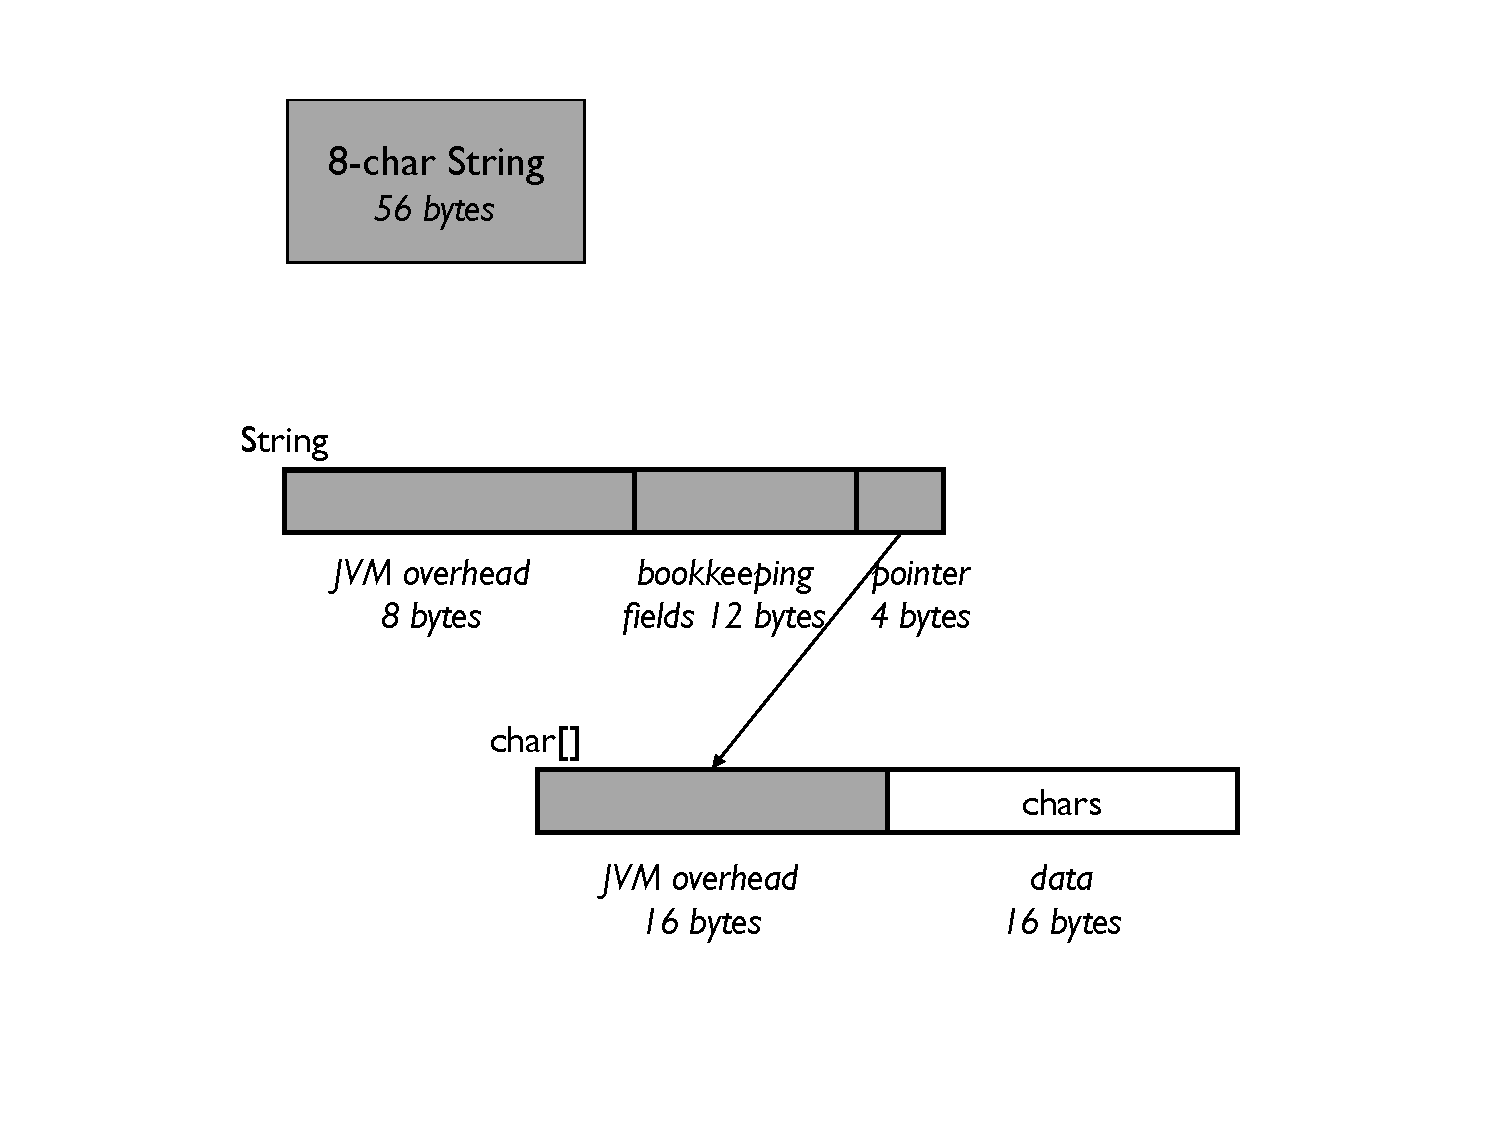
\includegraphics{eight-char-string}
  \caption{The cost of associating \class{UndateInfo} with every
  \class{ContactMethod}.}
  \label{fig:big-base-class}
\end{figure}
 
The solution in Figure~\ref{fig:big-base-class} provides a very fine
granularity of functionality. An argument can be made in favor of this
solution, since you lose functionality and flexibility if you only track
updates to \class{ContactPerson}. However, if the program hits a scalabity
problem, it may not be possible to be this casual with memory. Also, an alternate
design may be available that gives the desired functionality in a more memory-efficient way. In this
example, you could implement an update log instead of tracking updates in the objects themselves. Assuming
updates are sparse, this is a much better solution. It is very easy define a subclass without looking closely
at the memory size of its superclasses, especially if the inheritance chain is
long.


\section{Inner Classes}
[TODO: short section explaining that 1. there's a hidden this pointer in
non-static nested classes (i.e. in all three types of inner classes) and 2.
advise the reader to use static nested classes unless they need one of the other kinds.  Can
 reference Effective Java on the topic - he gives the same advice with
 additional arguments other than space.  The extra this pointer can also cause
 leaks/drag (example from Sun tutorial(?): a map entry nested class within a map.  
 Entry class is erroneously declared to be non-static).]

\section{Writing Efficient Framework Code}

The storage optimizations described in this chapter assume that you are
familiar with the entire application you are working on. You need to
understand how objects are created and used, and therefore know enough to determine
whether these optimizations make
sense. However, if you are programming a library or framework, you have no way
of knowing how your code will be used. In fact, your code may be used in a
variety of different contexts with different characteristics. Premature optimization ---
making an assumption about how the code will be used, and optimizing for that
case --- is a common pitfall when programming frameworks.  

For example, suppose the online store is designed as a framework
that can be extended to implement different kinds of stores.
For some stores, most products may have an alternate supplier. For other
stores, most products may not.  There is no way of knowing. If the
\code{Product} class is designed so that the alternate supplier is allocated as
a side object, then sometimes memory will be saved and sometimes wasted. 
One possibility is to define two versions of the \code{Product} class, one that
delegates and one that doesn't. The framework user can then use the version
that is appropriate to the specific context. However, this is generally not
practical. 

Frequently, decisions are made that trade space for time.
There are many instances of this trade-off in the Java standard library. For
example, let�s look at  \code{String}, which has three 
 bookkeeping fields, an offset,
a length, and a hashcode. These 12 bytes of overhead consume 21\% of an eight
character string. 
The offset and length fields implement an optimization for substrings. 
That is, when you create a substring, both
the original string and substring share the same character array, as shown in
Figure~\ref{fig:substring}. The offset and length fields in the substring
\code{String} object specify the shared portion of the character array. 
This scheme optimizes the time to create a substring, since there is no new
character array and no copying. However, every string pays the price of the offset
and length field, whether or not they are used.
Across all Java applications, there are many more strings than substrings, so a
lot of memory is wasted. Even when there are many substrings, if the original
strings go away, you have a different footprint problem, namely,
saving character arrays which are too big.
\begin{figure}
  \centering
 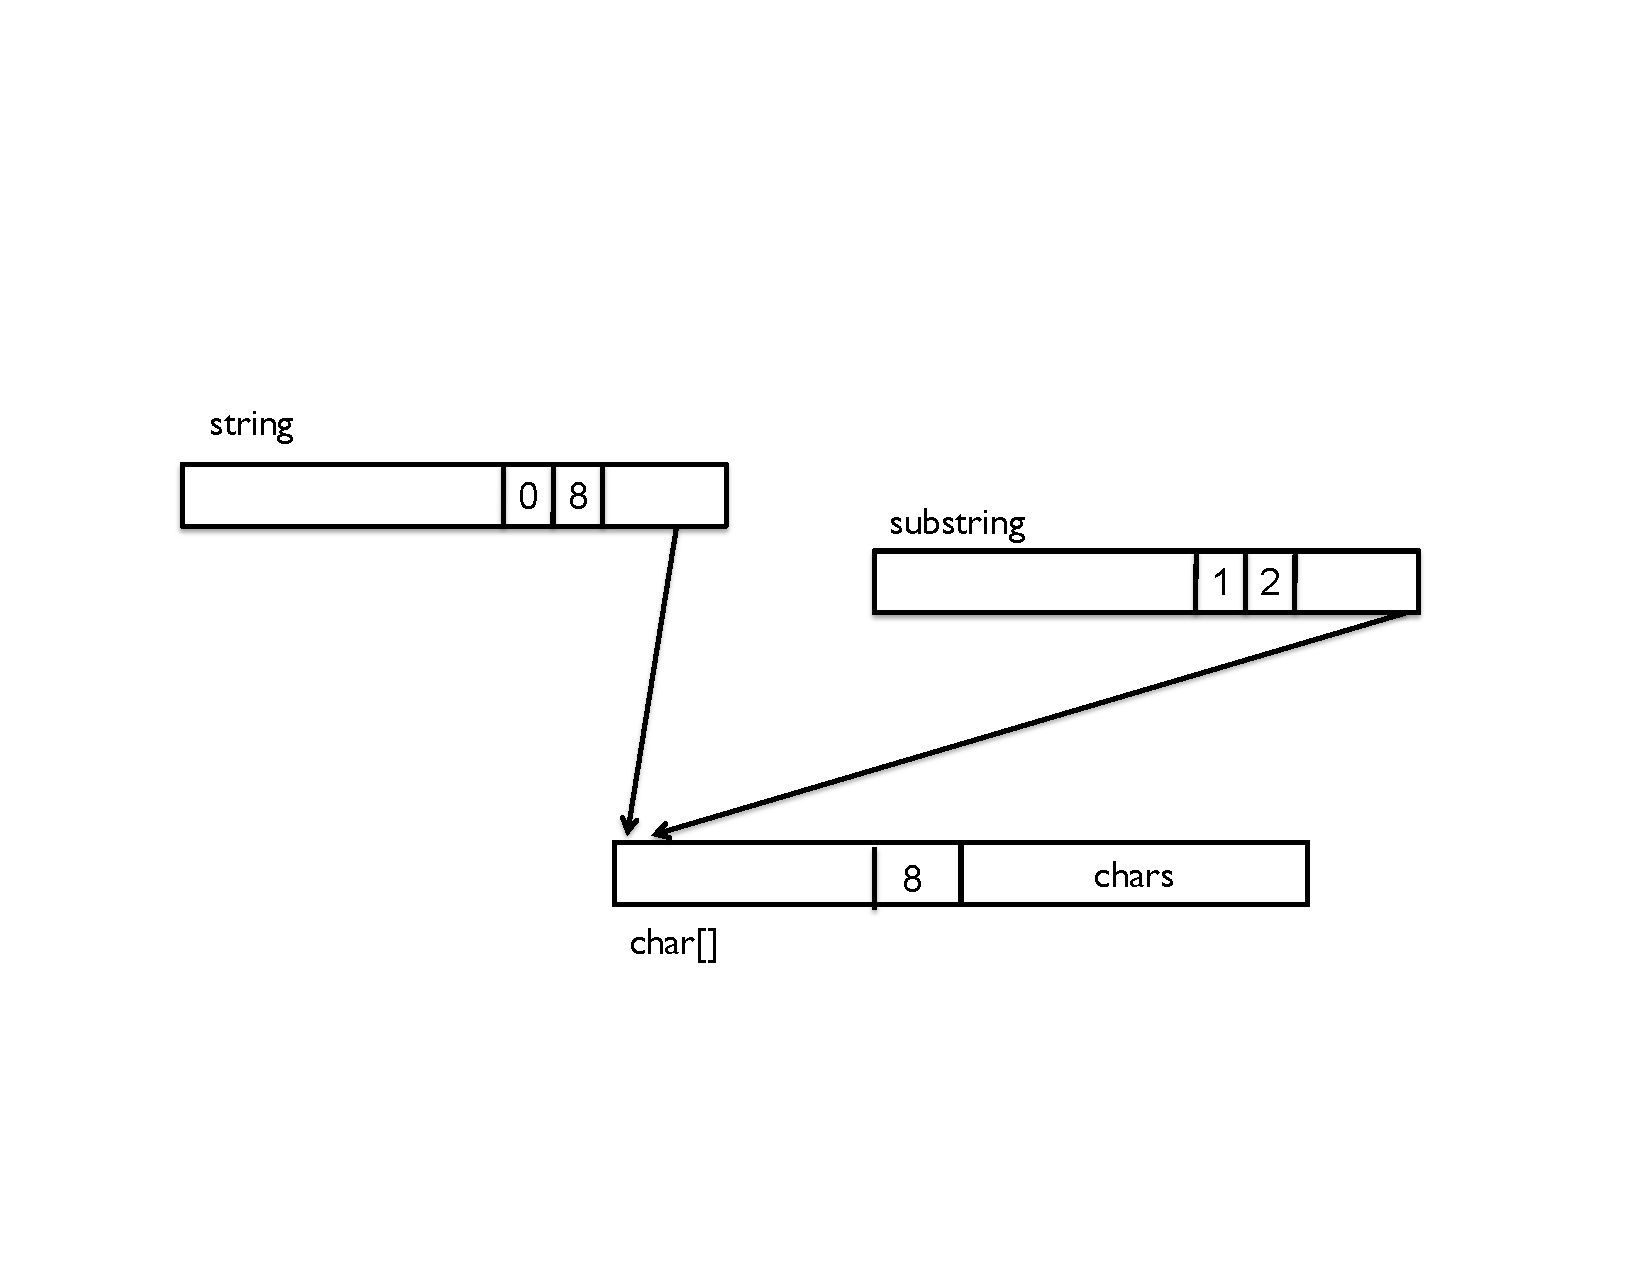
\includegraphics[width=.90\textwidth]{part1/Figures/modelingdatatypes/substring.pdf}
 % 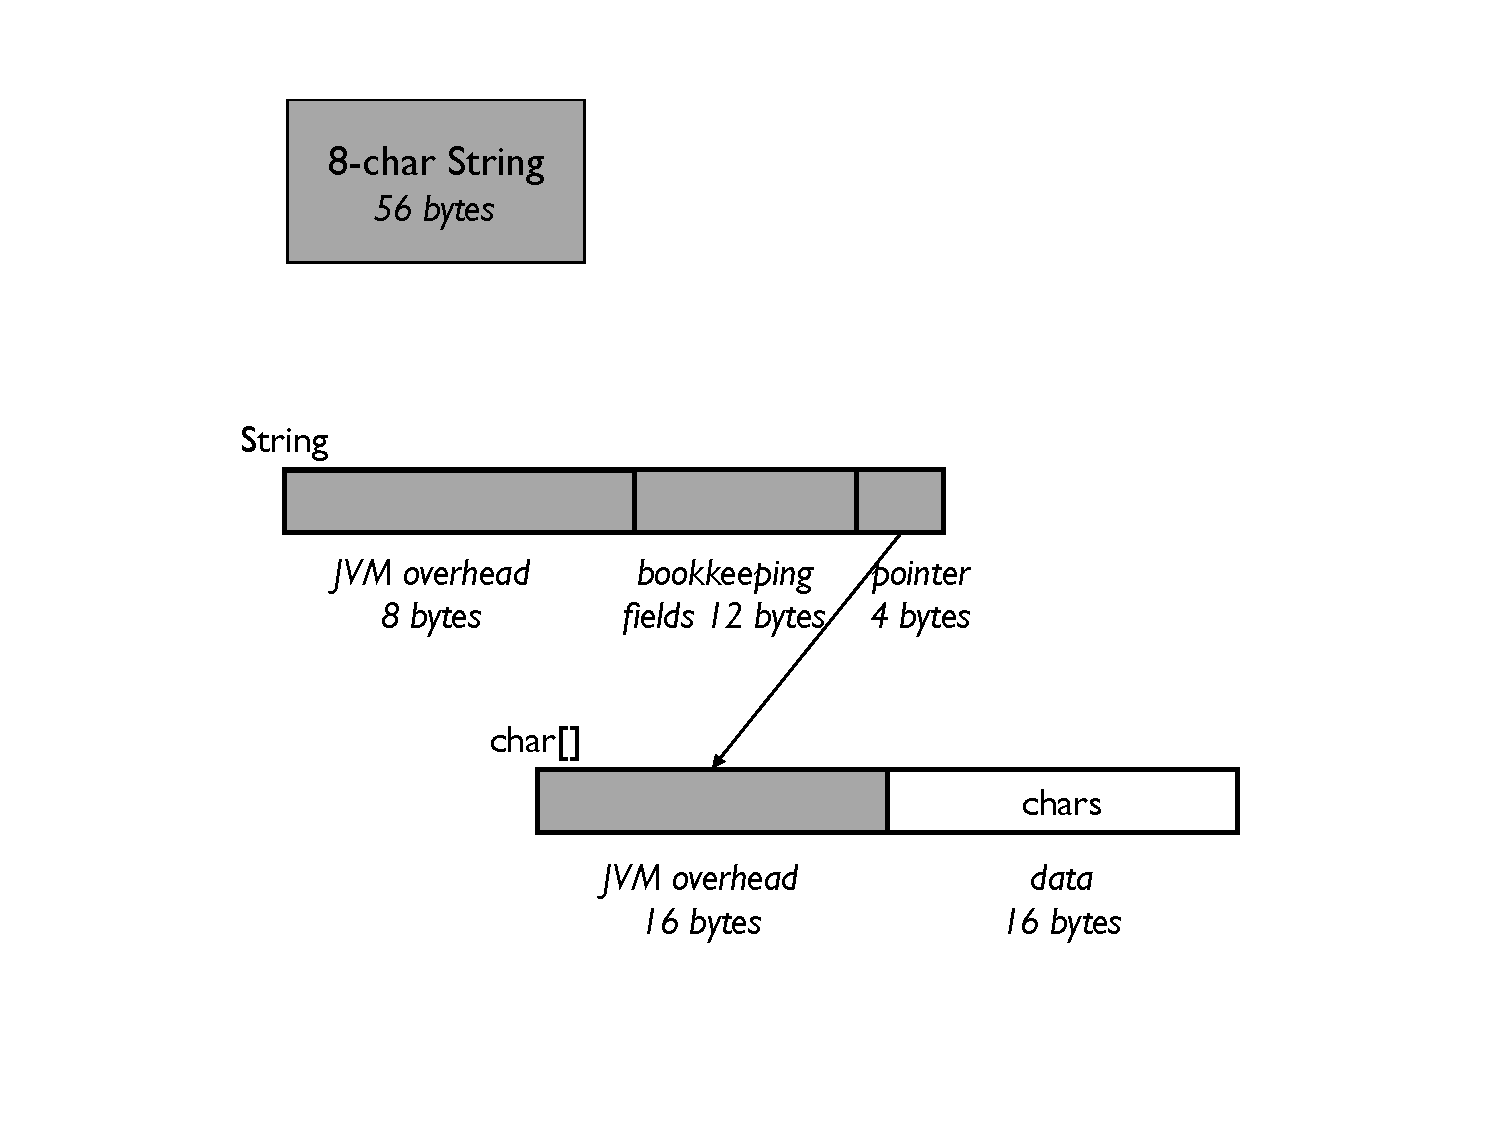
\includegraphics{eight-char-string}
  \caption{A string and a substring share the same character array. The length
  and offset fields are needed for the substring, but are redundant
  in the original string object.}
  \label{fig:substring}
\end{figure}

%It says that if I ever take a substring of this thing,
% I�m going to be able to share with the origjnal characters of the String This
 %is a theme you will see throughout the JDK, that there�s so many
% optimizations that are done to avoid copies at any cost. Really with a huge
% focus on time, and almost no focus on space whatsoever. So studies we saw at
% TRL, in reality, in the long liv

The third bookkeeping field in \code{String} is a hashcode.
Storing a hashcode seems like a reasonable idea, since it is expensive to
compute it repeatedly. However, you have to be puzzled by the space-time
trade-off, since 
a string only needs its hashcode when it is stored in a \code{HashSet} or a
\code{HashMap}. In both of these cases, the \code{HashSet} or \code{HashMap}
entry already has a field for hashcode for each element.
(As if this redundancy isn't enough, there are also four bytes reserved
in every object header for the identity hashcode.) 

This is a cautionary tale of premature optimization. Framework
decisions can have a long-lived impact. For these \class{String}
optimizations, it's not clear that there is any performance gain beyond 
some unrealistic benchmarks. 
But it's too late and expensive to change the implementation, 
so all applications must pay the price in memory footprint.

\section{Summary}

Even though Java does not let you control the layout of objects, it is still
possible to make objects smaller by recognizing certain usage patterns.
Optimization opportunities include:

\begin{itemize}
  \item Rarely used fields can be delegated to a side object, or stored in a
  completely separate attribute table.
  \item Fields that have the same value in all instances of a class can be
  declared static.
  \item Mutually exclusive fields can share the same field, provided they have
  the same type.
  \item Redundant fields whose value depends on the value of other fields can
  be eliminated, and recomputed each time they are used.
  \item 
\end{itemize}

Every field eliminated saves around 4 bytes per object, which may seem small.
However, often several optimizations can be applied to a class, and if the
class has the most objects in the heap, then these small optimizations turn out
to be significant. 

